\section{Delineamento}
\label{sec:orgd116b4d}
\subsection{As tarefas e os problemas de coordenação}
\label{sec:org8aaefd6}
\todo{Trecho vindo da introdução no corte de outubro de 2026, ainda por integrar a esta seção.}

O conjunto de tarefas é um \emph{benchmark} de notação, como os \emph{benchmarks}
de resultado qualitativo do projeto de linguagens
\cite[p. 35]{erdweg2015}, entre os quais está o 7GUIs
\cite[8:20]{lu2021}.

\begin{description}
\item[{Formulário com validação:}] os campos que dependem uns dos outros, o
estado derivado e o envio que, enquanto espera a resposta, ignora um
novo clique em Reservar, para o usuário não reservar o mesmo voo duas
vezes;
\item[{Busca com sugestões:}] o cancelamento da busca já requisitada, a resposta
anterior que nunca aparece e a lista derivada das sugestões, para o
usuário ver só as cidades correspondentes ao texto que está no campo;
\item[{Login com quarentena:}] a tentativa nova que cancela a anterior, para
o usuário que errou a senha tentar de novo sem esperar a resposta da
primeira, e o relógio da sessão, que para quando a sessão se encerra;
\item[{Quadro de tarefas:}] o estado compartilhado entre o cabeçalho e três
colunas, o limite de duas tarefas em "Fazendo", que desabilita os
botões das outras colunas, e o quadro gravado no navegador, para o
usuário achar cada tarefa na coluna em que a deixou, ao voltar à página
ou em outra aba;
\item[{Dados ao vivo:}] valores que uma fonte envia sem o usuário pedir, como
o placar de um jogo, a assinatura presa à tela e a pausa, para quem
acompanha o painel ler os valores sem que a tabela se atualize.
\end{description}

A orquestração pesa mais na Busca, no Login e nos Dados ao vivo, e o
gerenciamento de estado, no Formulário e no Quadro.
O Formulário adapta o \emph{Flight Booker}, uma das sete tarefas do 7GUIs, de
\textcite[p. 11 e 25]{kiss2014}, e acrescenta os campos de nome e de
e-mail.
O Login segue o painel de \textcite[p. 534]{berry2020}, e os Dados ao
vivo, as cotações que uma fonte empurra aos clientes, em
\textcite[p. 66]{meijer2012}.
\subsection{As tecnologias e os pares}
\label{sec:orga4f1a70}
\todo{Trecho vindo da introdução no corte de outubro de 2026, ainda por integrar a esta seção.}

Na web, Web Component, React e Solid, uma tecnologia por modelo de
programação, implementam as cinco tarefas.
O imperativo por atualização manual entra com o Web Component, a forma do
próprio navegador de criar elementos personalizados \cite{mozilla2026}.
Lit e Angular com \emph{signals} implementam três tarefas cada, em pares de
tecnologias próximas: o Lit com o Web Component, e o Angular com o Solid.
O Lit se constrói sobre o Web Component: seus componentes são elementos
personalizados do navegador, mas cada alteração de estado chama de novo o
método que monta a tela \cite{google2026d}.
Por isso fica no declarativo por re-renderização, como o React, com
outra notação.
O par Web Component e Lit, no Formulário, na Busca e nos Dados ao vivo,
mantém o modelo de componente e a orquestração.
Muda só a ligação do estado com a tela, escrita à mão no primeiro e
refeita pelo \emph{template} a cada alteração de estado no segundo.

No React e no Solid, a tela se monta em JSX, marcação parecida com \gls{html}
escrita dentro do JavaScript \cite{meta2026c}.
O que os separa, sobretudo, é o modo de coordenar: a cada alteração de
estado, o React reexecuta o componente inteiro, e o Solid atualiza só os
trechos da tela que dependem do \emph{signal} alterado
\cites[][ 289:38]{lee2025}{solidjs2026}.

Solid e Angular com \emph{signals}, ao contrário, coordenam do mesmo modo: os
dois guardam o estado em \emph{signals} e derivam valores de outros \emph{signals}
\cite{solidjs2026a,google2026}.
Por isso ficam no mesmo modelo de programação, e o par, no Formulário,
na Busca e no Quadro, mostra como a notação varia entre tecnologias em
três pontos.
No Solid, a tela se monta em JSX numa função, e, no Angular, num \emph{template}
baseado em \gls{html}, com construtos próprios \cite{google2026a}.
O componente do Angular é uma classe com decorador \cite{google2026b}, e
participa da injeção de dependências \cite{google2026c}.
E as \glspl{api} dos dois diferem no que vai além do \emph{signal} e do valor
derivado, como o cancelamento das requisições na Busca.
Quando o \emph{signal} se altera, o Solid recalcula só os valores e trechos da
tela que dependem dele \cite{solidjs2026}; o Angular marca o componente que o
lê e o atualiza na próxima detecção de alterações \cite{google2026}.

Dentro de um mesmo modelo de programação, a notação também muda de uma
tecnologia para outra, como entre o Solid e o Angular com \emph{signals} ou
entre o React e o Lit, e a avaliação registra quando essa diferença muda
a posição.

Fora da web, cada plataforma tem um par de tecnologias, que confere se
as posições encontradas na web se repetem em outra plataforma e outra
linguagem.
No Android, Views e Compose implementam o Formulário, o Quadro e os
Dados ao vivo.
As Views ficam no imperativo por atualização manual, e o Compose, no declarativo
por re-renderização, porque chama de novo as funções da tela quando o estado
se altera \cite{android2026}.
No \emph{desktop}, Windows Forms e WPF implementam o Formulário, o Quadro e o
Login.
O Windows Forms fica no imperativo por atualização manual, porque o
tratador de cada evento atribui os valores aos controles, sem o \emph{data
binding} que ele também oferece \cites{microsoft2025b}{microsoft2026a},
e o WPF, no declarativo por atualização granular, porque, quando um dado se altera, os elementos ligados a
ele se atualizam sozinhos \cite{microsoft2025}.

Na web, só o par Web Component e Lit isola o imperativo por
atualização manual, e só em três tarefas.
Ele isola a ligação do estado com a tela, e não a orquestração, que no
Lit se escreve como no Web Component.
Fora da web, os dois pares mudam também a montagem da tela, e cada
plataforma confere só dois dos três modelos de programação: o Android
fica sem o declarativo por atualização granular, e o \emph{desktop}, sem o
declarativo por re-renderização.
\subsection{As rodadas}
\label{sec:org3674dfb}
\todo{Trecho vindo da introdução no corte de outubro de 2026, ainda por integrar a esta seção.}

A avaliação se faz em três rodadas, cada uma mais estreita que a
anterior, como as de \textcite[p. 3]{kiss2014}: a primeira responde à
P1, e a segunda e a terceira, à P1.1 e à P1.2.
Na primeira rodada, as tecnologias implementam as tarefas descritas acima.
Na segunda, cada tarefa recebe funcionalidades, como o assistente
em três passos do Formulário, e requisitos de orquestração, como a
espera de 300 ms depois da última tecla na Busca.
Uma funcionalidade muda o que o usuário percebe ou pode fazer, e um
requisito de orquestração deixa a tela igual e muda só como se combinam
os eventos.
São onze mudanças, feitas uma por \emph{commit} e na mesma ordem em
todas as tecnologias que implementam a tarefa.
A segunda rodada faz o código crescer porque é nos problemas grandes que os efeitos
da viscosidade mais aparecem \cite[p. 161]{green1996d}.
Na terceira, o Formulário estendido é reescrito em cada tecnologia
com a biblioteca de formulário mais usada no ecossistema dela, ou com a
\gls{api} da plataforma quando nenhuma predomina.
Como as bibliotecas variam de uma tecnologia para outra, a conclusão da
terceira rodada vale para o ecossistema típico de cada tecnologia, e não só
para o modelo de programação.
\subsection{Os controles e o teste de conformidade}
\label{sec:org1c64492}
\todo{Trecho vindo da introdução no corte de outubro de 2026, ainda por integrar a esta seção.}

Quatro coisas poderiam diferenciar as implementações sem ser o modelo de
programação nem a notação, e as quatro ficam fixas: a linguagem, a
especificação, as bibliotecas e o domínio.
A linguagem é uma só em cada plataforma: na web, o \emph{TypeScript}, que o
Angular exige \cite{google2026b} e as demais tecnologias também usam; no
Android, o Kotlin; e, no \emph{desktop}, o C\#.
As implementações de uma tarefa seguem a mesma especificação, com os mesmos
textos, regras e dados, e, nas duas primeiras rodadas, cada uma usa só o que a própria
tecnologia traz, sem bibliotecas de formulário.
As regras que não dependem da interface, como o formato das datas, a
validação do e-mail e as transições do quadro, ficam num \emph{domínio} comum
às implementações de cada plataforma, na linguagem dela.
Esse controle das variáveis é parte do planejamento da pesquisa, o
delineamento \cite[p. 54]{prodanov2013}.

Um \emph{teste de conformidade} por tarefa executa as verificações da
especificação contra cada implementação; na web, ele roda no console do
navegador.
\emph{Capturas} de tela dos estados escolhidos de cada tarefa, geradas
automaticamente, denunciam desvios de comportamento ou de aparência,
porque devem sair idênticas entre as tecnologias web.
As implementações, os testes de conformidade e as capturas ficam num repositório público,
em \url{https://github.com/iquabius/unemat-tcc}.
Nele, as versões de linguagens, bibliotecas e ferramentas ficam
fixadas\footnote{No \texttt{package-lock.json} e no \texttt{libs.versions.toml}.
Na web, TypeScript 6.0.3, React 19.3.0, Solid 1.9.15, Lit 3.3.3 e Angular
22.2.0, com Vite 8.3.1 para o \emph{build} (no Angular, o \texttt{@angular/build} 22.2.0)
e Playwright 1.63.0 para as capturas.
No Android, Kotlin 2.4.20, Jetpack Compose pela \gls{bom}
2026.09.00 e, para as capturas, Robolectric 4.17 com Roborazzi 1.75.0.}, para que as implementações possam ser reproduzidas.
\subsection{A avaliação}
\label{sec:org63eabaa}
\todo{Trecho vindo da introdução no corte de outubro de 2026, ainda por integrar a esta seção.}

A avaliação cabe ao autor, que examina o código das implementações dimensão
a dimensão, sem participantes.
É uma avaliação analítica, feita por especialista, sem a participação de
usuários \cite{blandford2008}, como a de \textcite[p. 8]{kiss2014} pelas
\glspl{dc}.
Ela serve de alternativa aos estudos com programadores, que comparam
linguagens a custo alto e com resultados muitas vezes inconclusivos
\cite[p. 9]{sadowski2011}, e as \glspl{dc} pedem menos tempo que eles
\cite{dagit2006}.

Em cada rodada, a avaliação percorre as 14 \glspl{dc} da lista
completa \cite[p. 115-118]{blackwell2003}, e não um subconjunto
escolhido antes, porque a escolha prévia pode atrapalhar, e o conjunto
inteiro traz resultados inesperados e úteis \cite[p. 332]{blackwell2001}.
Para a análise, o trabalho as agrupa pelo que descrevem.
Oito tratam da notação: \emph{nível de abstração}, \emph{proximidade de
descrição}, \emph{consistência}, \emph{concisão}, \emph{operações mentais difíceis},
\emph{dependências ocultas}, \emph{expressividade de papel} e \emph{notação secundária}.
Duas são do sistema, que o ambiente de edição agrava ou atenua: a
\emph{viscosidade} e a \emph{propensão a erros}.
As outras quatro pesam no ambiente de edição: o \emph{compromisso
prematuro}, a \emph{avaliação progressiva}, a \emph{visibilidade} e a
\emph{provisoriedade}.
Destas, a avaliação lê a face que aparece na notação, porque os próprios
autores suspeitam que há uma zona cinzenta entre as dimensões da notação e as
do ambiente \cite[p. 357]{green2006}.
Nenhuma dimensão é boa ou má em si, e a avaliação sempre leva em conta a
atividade a apoiar \cite[p. 115]{blackwell2003}.
Na primeira rodada, as atividades são a busca e a compreensão exploratória
do código pronto, e, na segunda e na terceira, a modificação \cite[p. 113]{blackwell2003}.

A análise compara os modelos de programação pelo perfil
de cada um nas \glspl{dc} \cite[p. 106 e 112]{blackwell2003} e abre
com uma tabela-síntese, com uma linha por
\gls{dc} e uma coluna por modelo de programação.
Cada célula dá a posição do modelo na \gls{dc}, indica de que tarefa vem a evidência e
registra quando as duas tecnologias web da coluna divergem, o Solid e o
Angular com \emph{signals} ou o React e o Lit.
No primeiro par, ela diz também se a diferença vem da montagem da tela,
do modelo de componente ou da \gls{api}.
Como cada tarefa exercita problemas de coordenação próprios, a síntese
por problema reúne as células que vêm das tarefas dele.
Da primeira rodada para as outras duas, a linha de cada \gls{dc} diz se a diferença
entre os modelos de programação fica \emph{mantida}, \emph{ampliada}, \emph{reduzida},
\emph{anulada}, \emph{invertida} ou \emph{surgida}, e a célula diz se a posição do
modelo \emph{sobe}, \emph{desce} ou \emph{fica igual}.
Segue uma seção por \gls{dc}, com os trechos de uma tarefa escolhida,
antes da avaliação, pelo problema de coordenação que a dimensão mais toca.
Em cada seção, a análise aponta se a diferença está na coordenação, na
montagem da tela ou na ligação entre as duas.
Nas seções em que as tarefas do Android ou do \emph{desktop} mostram
diferença entre as duas tecnologias da plataforma, a análise diz se a
posição da web se repete nela.
A concisão tem ainda o apoio de uma contagem das linhas de cada
implementação.
Na segunda e na terceira rodada, o \emph{diff} de cada mudança apoia a viscosidade: a mesma
mudança, preparada antes e feita em cada implementação, como no teste
de \textcite[p. 162]{green1996d}, mostra quantas ações ela pede, e
quantas outras restauram a consistência \cite[p. 115]{blackwell2003}.
\section{Dimensões de avaliação}
\label{sec:orgbd22adb}
\todo{Trecho vindo da introdução no corte de outubro de 2026, ainda por integrar a esta seção.}
A avaliação usa as \glspl{dc}, que \textcite[p. 106]{blackwell2003} chamam de ferramentas
de discussão, para quem projeta ou avalia artefatos de informação, e não
de método analítico.

\textcite[p. 58 e 60]{blackwell2019} registram, na psicologia da
programação, o pedido por ensaios controlados randomizados no estudo do
projeto de linguagens e o ceticismo sobre apoiar nesse empirismo um
processo de projeto complexo.
Para eles, a parte cognitiva das \glspl{dc} importa bem menos que a teoria de
projeto implícita nelas.

As outras duas, \emph{expressividade} e \emph{operações mentais difíceis}, vêm do grupo
que \textcite[p. 15]{kiss2014} deixou de fora e que, a seu ver, teria
sido útil se as linguagens e os \emph{toolkits} comparados fossem muito mais
diferentes.
Na comparação principal, \textcite[p. 11-12]{kiss2014} escolheu o
ScalaFX porque este envolve o próprio JavaFX e porque o Scala é
sintaticamente próximo do Java.
Aqui, cada tecnologia traz as próprias abstrações, e as três notações
diferem na forma de escrever a coordenação.
E, ao avaliar bibliotecas reativas, ele próprio descreve o esforço
mental de cada uma sem uma dimensão para isso
\cite[p. 87 e 97]{kiss2014}.

As duas tratam da leitura do código.
A expressividade é a facilidade de reconhecer o propósito de cada
trecho, e as operações mentais difíceis obrigam quem lê a contar nos
dedos ou anotar à parte para acompanhar o que acontece \cite{green1996d}.
Ao avaliar se quem lê entende uma especificação,
\textcite[p. 267]{britton2001} também as incluíram entre as dimensões
especialmente úteis.
Na comparação de \textcite{mernik2009} entre o \gls{xaml} e o C\# Forms, as duas
estiveram entre as dimensões que mais pesaram na compreensão dos
programas.

As outras três do grupo ficam de fora.
O compromisso prematuro nasce da ordem em que o ambiente de edição obriga a
construir o programa, e o código pronto não guarda essa ordem
\cite{green1996d}.
A consistência mede o quanto quem aprende consegue adivinhar da notação,
e só se avalia por introspecção \cite{green1996d}.
Já a notação secundária (comentários, indentação e nomes) é própria de
quem escreve \cite{green1996d}.
Aqui, ela é padronizada entre as tecnologias, e por isso não distingue
uma notação da outra.
As dimensões utilizadas neste trabalho são baseadas nas \glspl{dc} de
\textcite{green1989}. Assim usamos critérios estabelecidos, o que facilita a
comparação de nossos resultados com trabalhos baseados nas \glspl{dc}. O \emph{framework}
completo possui 14 dimensões, mas os autores recomendam usar um subconjunto
apropriado para o artefato em mãos.

\begin{description}
\item[{Nível de abstração}] \emph{Disponibilidade e tipos de mecanismos de abstração}

O sistema fornece alguma forma de definir novos termos com a notação pra
que eles possam ser extendidos afim de descrever ideias claramente? Os
detalhes podem ser encapsulados? O sistema insiste em definir novos
termos? Qual o número de novos conceitos de alto nível devem ser
aprendidos pra se fazer uso do sistema? Eles são fáceis de aprender e
usar?

   Cada novo conceito é um empecilho pra aprendizagem e aceitação, mas
também pode tornar um código complexo mais compreensível. Por exemplo, o
React emprega o \emph{fluxo de dados de mão única} --- do inglês \emph{one-way data
flow} ou \emph{one-way binding} --- em sua arquitetura. É necessário aprender
conceitos novos para usar os componentes do React de forma adequada. Não
compensa para aplicações pequenas, mas para aplicações complexas pode tornar
o código mais compreensível e passível de manutenção porque os detalhes
podem ser encapsulados em novos termos: os componentes.

Outro exemplo é a função:

\begin{citacao}
  A function has a name and, optionally, parameters as well as a body that
  returns a value following certain computational steps. A client can simply
  refer to a function by its name without knowing its implementation details.
  Accordingly, a function abstracts the computational process involved in the
  computation of a value. The learning barrier to the principle of a function is
  not great but it can still make a lot of code much more understandable 3 by
  hiding unimportant details.
  \cite[p.~13]{kiss2014}
\end{citacao}

\item[{Proximidade de descrição}] \todo{Traduzido de “Closeness of mapping”, poderia ser “Proximidade de mapeamento”} \emph{Semelhança entre representação e o domínio}

O quão relacionado é a notação com o resultado que ela descreve, ou
melhor, o domínio do problema? Que partes parecem ser uma forma
particularmente estranha de descrever algo?

\begin{citacao}
  Um exemplo é a definição de layout de uma interface gráfica. Linguagens que
  não fornecem uma forma de descrever o layout de modo aninhado, ou seja,
  hierárquico, e como tal força o programador a “linearizar” o código com o uso
  desnecessário de variáveis intermediárias, dificultando enchergar como a
  estrutura de definição do layout corresponde com o layout final da aplicação.
  Não é atoa que especificações baseadas no XML são amplamente usadas na
  construção de interfaces gráficas em linguagens sem suporte nativo para
  representação hierárquica de layout.
  \cite[p.~13; tradução nossa]{kiss2014}
\end{citacao}

\item[{Dependências ocultas}] \emph{Vínculos importantes implícitos entre entidades}

As dependências entre as entidades da notação são visíveis ou ocultas?
Todas as dependências são especificadas em ambas as direções? Alterações
locais podem ter efeitos globais confusos?

Se uma entidade cita outra, que por sua vez cita uma terceira, a
alteração do valor da terceira entidade pode desencadear efeitos
inesperados. O principal problema não é o fato de A depender de B, mas sim
que a dependência não é explicitamente visível. Um caso bem conhecido de dependência
oculta é o “problema da classe base frágil”\footnote{Veja: \url{https://en.wikipedia.org/wiki/Fragile\_base\_class}.}.

\begin{citacao}
  In (complex) class hierarchies a seemingly safe modification to a base class
  may cause derived classes to malfunction. The IDE in general cannot help
  discovering such problems and only certain programming language features can
  help preventing them. Another example are non-local side-effects in
  procedures, i.e. the dependencies of a procedure with non-local side-effects
  are not visible in its signature.
  \cite[pg.~14]{kiss2014}
\end{citacao}

\item[{Propensão a erros}] \emph{Notação incita erros}

Até que ponto a notação influência o programador a cometer um erro? Fazer
algumas coisas parece ser particularmente complexo ou difícil, p. ex.,
juntar várias coisas?

Em muitas linguagens dinâmicas com definições implícitas de
variáveis\footnote{Isto é, quando não se precede uma definição de variável
com \texttt{var} ou \texttt{let} por exemplo.}, um erro de tipagem em uma variável pode
de repente causar erros difíceis de encontrar já que o \gls{ide} nem sempre
pode apontar tal erro devido a dinamicidade na linguagem. A inicialização
implícita de variáveis com valor \texttt{null} pode levar a uma exceção de
ponteiro nulo se o programador esquecer de inicializar as variáveis
corretamente antes de usá-las.

\item[{Concisão        }] \emph{Verbosidade da linguagem}

Quantos símbolos ou quanto espaço a notação requer pra produzir um certo
resultado ou expressar uma ideia. Que tipos de coisas ocupam mais espaço
para se descrever?

\begin{citacao}
  Some notations can be annoyingly long-winded, or occupy too much valuable
  “real-estate” within a display area. In Java before version 8 in order to
  express what are lambdas today anonymous classes were employed. Compared to
  Java 8’s lambdas these anonymous classes used to be a very verbose way of
  encoding anonymous functions especially when used in a callback-heavy setting
  like traditional GUI programming~\cite[p.~14]{kiss2014}.
  \todo[inline]{Pensar num exemplo mais próximo da Web e substituir citação direta.}
\end{citacao}

\item[{Viscosidade    }] \emph{Resistência a mudanças}

Existe alguma barreira contra mudança na notação? Quanto esforço é
necessário pra fazer uma alteração num programa expresso na notação?

Num sistema viscoso o usuário precisa realizar várias passos para
concluir uma tarefa. Alterar o tipo de retorno de uma função pode causar
erros em várias partes do código onde a função é chamada. Nesses casos um
\gls{ide} pode ajudar muito.
\end{description}


Outras dimensões que ficaram de fora são:

\begin{itemize}
\item Comprometimento prematuro: \emph{limitações na ordem de fazer as coisas}
\item Expressividade: \emph{o propósito de uma entidade pode ser rapidamente determinado}
\item Consistência: \emph{semânticas parecidas são apresentadas em estilo sintático
parecido}
\item Operações mentais difíceis: \emph{alto esforço cognitivo pra realizar tarefas}
\item Notação secundária: \emph{informações extras por meio de notações além das
formais}
\end{itemize}
\todo[inline]{Berndt sugeriu considerar “Expressividade” e “Operações mentais difíceis”.}

Em outras situações, e dependendo dos artefatos de informação, essas dimensões
poderiam ser úteis. Se tivéssemos focado mais nas ferramentas e no processo de
construção dos estudos de caso então as seguintes dimensões poderiam ser usadas:

\begin{itemize}
\item Visibilidade: \emph{habilidade de ver os componentes claramente}
\item Análise progressiva: \emph{trabalho realizado pode ser verificado em qualquer
momento}
\item Provisoriedade\todo{'momentaneidade' ou 'transitoriedade'}: \emph{grau
de comprometimento com uma ação ou marco}
\end{itemize}
\section{*Revisão do JavaScript}
\label{sec:orga965f6a}
Talvez devêssemos colocar uma seção de revisão das ferramentas utilizadas na
implementação dos estudos de caso? Poderíamos descrever os recursos relevantes
para nossa análise.
\todo[noline]{Berndt disse p/ colocar como apêndice}
\section{Processamento de listas}
\label{sec:org2c421db}

Uma coleção é um agrupamento com uma quantidade variável de itens, que (1)
compartilham algum significado ao problema a se resolver e (2) precisam ser
manipulados juntos de forma controlada.

O único tipo de coleção no JavaScript é o arranjo, ou \emph{array}, que pode ser
construído através do objeto\footnote{Diferente da maioria das linguagens, em que objetos são
instâncias de classes, no JavaScript os objetos são extensões de \emph{protótipos}.} global \mintinline{js}{Array}, ou da
notação de arranjos literais com colchetes:

\begin{listing}[htbp]
\caption{Criando coleções}
\begin{minted}[]{js}
var collection1 = new Array();
var collection2 = [];
\end{minted}
\end{listing}

Uma tarefa muito comum na programação é a iteração\footnote{O processo de percorrer, um por um, os itens de uma coleção.} de coleções.
Um mecanismo muito utilizado para tal é o comando \mintinline{js}{for}. Em
\ref{code:forLoopTraverse} é demonstrado o uso do comando \mintinline{js}{for} para
percorrer os itens da coleção \mintinline{js}{people} e mostrar cada um no console de
depuração.

\begin{listing}[htbp]
\caption{\label{code:forLoopTraverse}Percorrendo uma coleção com o laço \mintinline{js}{for}}
\begin{minted}[]{js}
var people = ["Alan Turing", "Alonzo Church", "Kurt Gödel"];
var count  = 0;

for (count = 0; count < people.length; count++) {
  console.log(people[count]);
}
\end{minted}
\end{listing}
\subsection{Formatação de preços}
\label{sec:org88a145a}

Nesta seção veremos como formatar uma lista preços para serem mostrados na
tela, p. ex., transformando um valor numérico \mintinline{js}{50.45} em uma \emph{string}
\mintinline{js}{"R$ 50.45"}. Para isso usamos uma função de formatação que é aplicada
a cada valor da lista. A função de formatação pode ser observada em
\ref{code:formatPriceFunction}.

\begin{listing}[htbp]
\caption{\label{code:formatPriceFunction}Função pra formatar um preço}
\begin{minted}[]{js}
function formatPrice(price) {
  return 'R$' + price.toFixed(2);
}
\end{minted}
\end{listing}

Em \ref{code:formatPricesFor} pode-se ver a solução implementada com o laço
\mintinline{js}{for}.

\begin{listing}[htbp]
\caption{\label{code:formatPricesFor}Formatação de preços com laço \mintinline{js}{for}}
\begin{minted}[]{js}
const prices = [50.45, 47, 20.99, 3.44, 1];
let formatedPrices = [];

for (let i = 0; i < prices.length; i++) {
  formatedPrices.push(formatPrice(prices[i]));
}
\end{minted}
\end{listing}

Em \ref{code:formatPricesMap} pode-se ver a solução implementada com a função
\mintinline{js}{map}.

\begin{listing}[htbp]
\caption{\label{code:formatPricesMap}Formatação de preços com laço \mintinline{js}{for}}
\begin{minted}[]{js}
const prices = [50.45, 47, 20.99, 3.44, 1];

const formatedPrices = prices.map(formatPrice);
\end{minted}
\end{listing}

Outras ideias:

\begin{itemize}
\item Adicionar \(1\) a cada número de uma lista
\item Multiplicar os números de uma lista
\item Transformar palavras com letras minúsculas de uma lista em palavras com
letras maiúsculas
\end{itemize}
\subsection{Seleção de valores com \texttt{filter()}}
\label{sec:orga71909e}
Remover nomes que não começam com ‘S’
\subsection{Nivelamento de valores com \texttt{concatAll()}}
\label{sec:org378b379}
\subsection{Redução de valores com \texttt{reduce()}}
\label{sec:org4b34d80}

O método \mintinline{js}{reduce()} executa uma função \textbf{reducer} para cada item da
lista, resultando num único valor. Em \ref{code:somaDePreçosComReduce} é
demostrado a soma dos preços de uma lista usando o método \mintinline{js}{reduce()}.
Nesta demonstração a função \mintinline{js}{somar()} é o \textbf{reducer}.

\begin{listing}[htbp]
\caption{\label{code:somaDePreçosComReduce}Soma dos preços de uma lista com o método \mintinline{js}{reduce()}.}
\begin{minted}[]{js}
const preços = [50.45, 47, 20.99, 3.44, 1];

const somar = (a, b) => a + b;
const total = preços.reduce(somar);
\end{minted}
\end{listing}
\subsection{Agrupamento de valores com \texttt{zip()}}
\label{sec:org0bf671c}
\section{Coordenação de eventos}
\label{sec:org48c8456}
\todo{Trecho vindo da introdução no corte de outubro de 2026, ainda por integrar a esta seção.}
A triagem em geral se apoia no que se escreveu sobre as alternativas, e não
no uso delas \cite[p. 15]{kitchenham1996}.
Aqui, ela se apoia também no uso de duas das notações, porque o autor
escreveu implementações de referência em React e em JavaScript com
\emph{callbacks}.
Na escrita das implementações, a familiaridade desigual do autor pesa
menos, porque elas seguem a mesma especificação e são padronizadas entre
as tecnologias.

\textcite[p. 11]{kiss2014} também compara as implementações pela
usabilidade do código, e não por tempo de execução e memória, como num
\emph{benchmark} tradicional.

O jQuery e o Web Component derivam a Lista filtrável com \texttt{filter}, \texttt{sort} e
\texttt{map}, funções de \gls{pf}.
E o React e o Solid recorrem a efeitos para sincronizar o componente com
sistemas externos, como o armazenamento do navegador no Carrinho.
A documentação do React chama os efeitos de “uma saída de emergência do
paradigma do React” \cite[tradução nossa]{meta2026b}.

Três das cinco tarefas partem do 7GUIs \cite[p. 17, 25 e 34]{kiss2014}:

\begin{description}
\item[{Contador}] a tarefa \emph{Counter};
\item[{Formulário com validação}] a \emph{Flight Booker}, ampliada com os campos de
um formulário real;
\item[{Lista filtrável}] o filtro por prefixo da tarefa \emph{Crud}.
\end{description}

O \emph{Timer} trata da concorrência entre um relógio e o usuário, mas nenhuma
das sete tarefas faz uma requisição cujas respostas chegam fora de ordem ou
são canceladas \cite[p. 30]{kiss2014}.
E nenhuma põe três componentes independentes para ler e alterar o mesmo
estado, como os do Carrinho.

No React, um valor derivado é uma expressão comum, recalculada a cada
execução do componente \cite{meta2026b}.
No Solid, é uma função que lê o \emph{signal} \cite{solidjs2026a}.

No Android, as duas variantes são escritas em Kotlin, a linguagem que o
Android recomenda e a única em que o Compose se escreve \cite{android2026a}.
O domínio em Kotlin responde diferente do da web em entradas-limite, como
anos de 0 a 99, e cada diferença conhecida fica registrada num teste.
Entre Views e Compose, a única diferença admitida nas capturas é a de
poucos pixels na renderização do texto.
\subsection{Contador}
\label{sec:org9fb74d8}

\begin{description}
\item[{Problema}] entender os conceitos essenciais da linguagem e a estrutura
básica necessária
\end{description}

\begin{figure}[htbp]
\caption{\label{img:contador}Interface gráfica do Contador.}
\centering
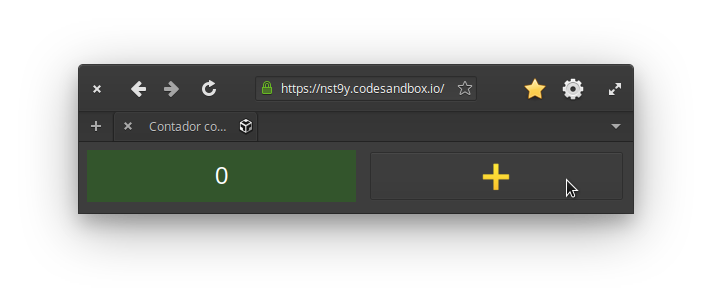
\includegraphics[width=12cm]{./fig/screenshot-contador-epiphany.png}
\end{figure}

A implementação do contador usando classes poder ser observado em
\ref{code:contadorComPOO}.

\begin{listing}[htbp]
\caption{\label{code:contadorComPOO}Contador com POO.}
\begin{minted}[]{js}
// No Java isto extenderia alguma classe padrão do toolkit,
// como `Application`
class Contador {
  constructor(props) {
    // Em Java estas propriedades precisam ser definidas antes
    this.contador = props.valorInicial;
    this.caixaDoValor = document.getElementById("valor");
    this.botãoDeIncrementar = document.getElementById("botãoDeIncrementar");
    this.botãoDeIncrementar.addEventListener(
      "click",
      // Isto requer uma explicação um tanto extensa
      this.tratarClique.bind(this)
    );
  }

  tratarClique(_evento) {
    this.contador = this.contador + 1;
    this.renderizar();
  }

  // Equivalente ao `public static void main()` do Java
  renderizar() {
    this.caixaDoValor.innerText = this.contador;
  }
}

const contador = new Contador({ valorInicial: 0 });
// Como no Java o `main()` é padronizado, sua execução seria
// feita automaticamente pelo ambiente de execução.
contador.renderizar();
\end{minted}
\end{listing}

O \mintinline{js}{tratarClique.bind(this)} na linha 12 requer uma explicação um tanto
extensa.

O contador usando função e operadores do xstream pode ser observado em
\ref{code:contadorComPR}.

\begin{listing}[htbp]
\caption{\label{code:contadorComPR}Contador com PR.}
\begin{minted}[]{js}
import fromEvent from "xstream/extra/fromEvent";

const Contador = props => {
  const caixaDoValor = document.getElementById("valor");
  const botãoDeIncrementar = document.getElementById("botãoDeIncrementar");

  // Fluxo que emite um evento toda vez que o botão for clicado
  const cliqueStream = fromEvent(botãoDeIncrementar, "click");

  // Fluxo que emite "valor + 1" (acumulado) toda vez que
  // cliqueS emite um evento
  const contadorStream = cliqueStream.fold(
    (valor, _evento) => valor + 1,
    props.valorInicial
  );

  const observador = {
    next: valor => {
      caixaDoValor.innerText = valor;
    }
  };

  contadorStream.addListener(observador);
};

Contador({ valorInicial: 0 });
\end{minted}
\end{listing}
\subsubsection{Análise}
\label{sec:org5d44f35}

Essa primeira análise é focada no básico.
\paragraph{Nível de abstração}
\label{sec:orgc19e1d8}
Na solução com \gls{poo} os conceitos da linguagem que deve-se entender são:
classes, construtor, objetos, propriedades, métodos, \emph{callbacks} na forma
de método, e conhecimento da \gls{api} do objeto do documento do \gls{html} ---
\gls{dom}.
Além do caso do \mintinline{js}{this} específico do JavaScript:
\mintinline{js}{this.tratarClique.bind(this)}.
Embora sejam conceitos básicos para um programador experiente em JavaScript
e \gls{poo}, o número é grande.
Abstrações mais sofisticadas não são necessários pelo Contador e o sistema
não insiste em abstrações especiais.
Apesar da solução usar uma quantidade considerável de conceitos, eles são
básicos, então observamos que o Nível de Abstração é baixo, ou seja, bom.

Em contrapartida, na solução com \gls{pr} os conceitos usados são: funções,
variáveis, fluxos e eventos, callbacks, e a \gls{api} do \gls{dom}.
A abstração mais sofisticada é o método \mintinline{js}{fold()} do fluxo de evento,
que nada mais é que uma versão assíncrona do \mintinline{js}{Array.reduce()}
nativo --- veja a soma de preços em \ref{code:somaDePreçosComReduce}.
Ambos produzem um resultado para cada elemento da lista.
A diferença é que no primeiro a lista é de eventos assíncronos, e infinita.
No segundo a lista é síncrona, com valores escales (números, \emph{strings},
objetos, etc.).
\todo{Paralelo entre métodos assíncronos e síncronos em outra seção?}
Níveis mais altos de abstração não são necessários, então a solução com \gls{pr}
é igualmente boa ou um pouco melhor que a solução com \gls{poo} quanto ao Nível
de Abstração.
\paragraph{Proximidade de descrição}
\label{sec:orga47cd1b}
Essa dimensão/critério faz mais sentido para análise de apresentação do que
comportamento (coordenação de eventos).
\paragraph{Dependências ocultas}
\label{sec:org9672d36}
\todo[noline]{Acredito que o HTML só não está situado no mesmo local que o código JavaScript, que é diferente de “oculto”.}
As únicas dependências que podem ser consideradas ocultas são os elementos
\gls{html} buscados pelo identificador com \texttt{document.getElementById("id")}.
\paragraph{Propensão a erros}
\label{sec:orgcf1dbd8}
Na solução com \gls{poo}, esquecer de vincular a instância do contador à função
\texttt{tratarClique()} resultará no erro “TypeError: this.renderizar is not a
function”.
Pois o valor do \texttt{this} estará vinculado ao objeto que chamou
\texttt{tratarClique()}, ou seja, o \texttt{this.botãoDeIncrementar}.
\todo{Talvez isso seja uma dependência oculta?}
Isso se deve ao fato de a palavra chave \texttt{this} se comportar de forma
diferente no JavaScript quando comparado com outras linguagens.

\begin{quote}
In most cases, the value of this is determined by how a function is called
(runtime binding). It can't be set by assignment during execution, and it
may be different each time the function is called. ES5 introduced the
bind() method to set the value of a function's this regardless of how it's
called, and ES2015 introduced arrow functions which don't provide their own
this binding (it retains the this value of the enclosing lexical context).
\cite{This2020}.
\end{quote}

\todo[inline]{Nos próximos exemplos acredito que podemos usar as funções de seta
  como callback no lugar dos métodos, pois possuem o valor do this vinculado
  lexicalmente. O Java possui lambdas desde a versão 8, o que despensa o uso de
  métodos para casos como esse. Ou já removemos desse primeiro? Pra evitar ter
  que explicar o \texttt{.bind(this)} que é um problema específico do
  JavaScript}.

Na solução com \gls{pr}, esquecer de definir o observador fará com que a
\texttt{caixaDoValor} não seja atualizada.
Pois ela não será renderizada, apesar de toda a lógica do contador
funcionar.
Apesar de tudo, essas possibilidades de erros não são críticas.
\paragraph{Concisão}
\label{sec:org26eab14}
Na solução com \gls{poo} o método \mintinline{js}{tratarClique()}, usado como \emph{callback},
poderia ser substituído por uma função de seta.
Além de poupar algumas linhas o uso do \mintinline{js}{.bind(this)} se torna
desnecessário.
Veja o código do Contador com \gls{poo} e função de seta em
\ref{code:contadorComPOOeFuncDeSeta} no apêndice.
Na solução com \gls{pr} a variável intermediária \mintinline{js}{contadorStream} poderia ser
removida, encadeando a chamada do \mintinline{js}{fromEvent} com o \mintinline{js}{fold()}:
\mintinline{js}{const cliqueStream = fromEvent().fold()}.
No entanto essa manobra diminuiria a legibilidade do
código\footnote{Note que o nome da variável \mintinline{js}{cliqueStream} já nem faz mais
sentido, pois o resultado da expressão não inclui apenas os eventos de clique.}.
De qualquer forma, a \gls{pr} evita a verbosidade da declaração da classe e dos
métodos, além da repetição do \mintinline{js}{this}.
Então em termos de Concisão a \gls{pr} está à frente da \gls{poo}.
\paragraph{Viscosidade}
\label{sec:org1b0eb09}
Num caso tão simples como o do Contador a única resistência a alteração
está em renomear atributos no caso da \gls{poo}, e variáveis na \gls{pr}.
No entanto isso é inevitável ao renomear termos.
Além disso o \gls{ide} pode ajudar através de uma funcionalidade de refatoração.
\todo{Talves seja interessante analisar a viscosidade da alteração pra colocar um botão de decremento (-1) do Contador.}
\subsection{Reserva de voo}
\label{sec:orgae3464c}
